\section{Obecný návrh sítí}
\label{sec:Chapter42}
V každém bloku se nachází dvě konvoluční operace o velikosti filtru $3\times3$, jednotným krokem v obou směrech os a ReLU aktivační funkcí. Pro všechny konvoluční operace bylo aplikováno místo odsazení typu valid padding odsazení typu same padding oproti původní architektuře \cite{unet} pro zachování velikosti obrazu na vstupu a výstupu sítě jako celku.

Pro konvoluční vrstvy s aktivační funkcí ReLU byly použity kernelové inicializéry typu \textit{He Normal}, které jsou často používány pro vrstvy s aktivační funkcí ReLU \cite{relu_henormal} a je to také i konzistentní nastavení s například oficiální implementací U-Net++ \cite{unetpp_github}. 

V blocích enkodéru se v naší implementaci používá $2\times2$ vrstva typu max pooling a $2\times2$ vrstva typu up-sampling zase v blocích dekodéru. Vrstva typu up-sampling tvoří náhradu pro původní vrstvu typu transpose. Toto rozhodnutí prane z úsudku založeném na uspokojivých výsledcích experimentálních modelů. 

\begin{figure}[ht]
    \centering
    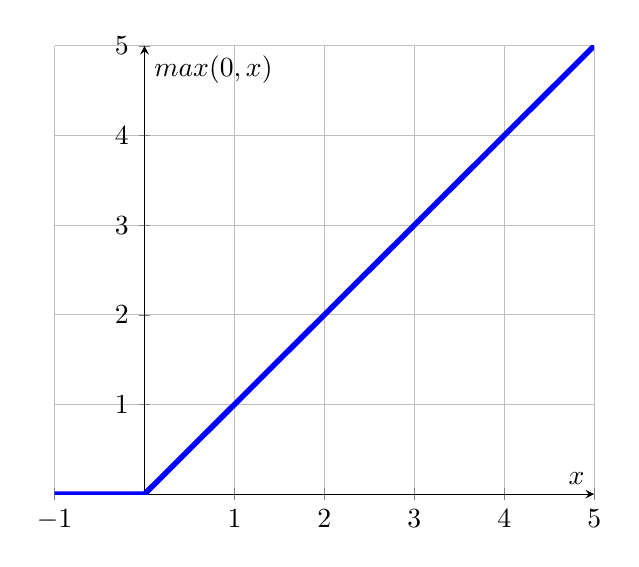
\begin{tikzpicture}
    \begin{axis}[
        axis lines=middle,
        xlabel={$x$},
        ylabel={$max(0, x)$},
        ymin=0, ymax=5,
        xmin=-1, xmax=5,
        xtick={-1,0,...,5},
        ytick={0,1,...,5},
        grid=major,
    ]
    
    \addplot[blue,line width=2pt] {max(0, x)};
    \end{axis}
    \end{tikzpicture}
    \caption[Aktivační funkce ReLU]{Aktivační funkce ReLU}
    \label{fig:relu}
\end{figure}

Pro každou z 2 konvolučních vrstev v rámci bloku bylo rozhodnuto aplikovat dávkovou normalizaci (ang. batch normalization), jelikož byl dokázán její pozitivní vliv ve většině případů v sítích U-Net \cite{unetnormalization}. Dávková normalizace je aplikována po konvoluční operaci a před aktivační funkcí. Dávková normalizace nebyla aplikována po finální výstupní $1\times1$ konvoluční vrstvě, a to na základě úvahy představení možného detrimentálního efektu na poslední trénovatelnou část sítě generující finální mapu příznaků, kde již nenásleduje žádná další vrstva.

Finální vrstva sítě je navržena pomocí $1\times1$ konvoluční operace na finálním bloku dekodéru. Finální vrstva má na výstupní mapě příznaků původní výšku a šířku vstupního snímku sítě, což je dosaženo pomocí aplikace odsazení typu same padding. Výstup generuje separátní mapy příznaků pro každou třídu klíčových bodů, kterých je v této práci 11. Dále v této práci jsou tyto výstupní mapy příznaků referovány jako výstupní kanály.

Pro učení se používá Gaussova funkce s pevně nastavenou hodnotou $\sigma$ a je to i výstupem trénovatelné části sítě. Detailní informace týkající se výstupu sítě a sítí následujících v této práci je detailněji popsáno v kapitole \ref{sec:Chapter46}.
\endinput